\documentclass[a4paper,twoside, twocolumn, 11pt]{article}
\usepackage{a4wide,graphicx,subfigure,fancyhdr,amsmath,amssymb,enumerate,hyperref, float,appendix}
\usepackage[english]{babel}
\numberwithin{equation}{section}

%----------------------- Macros and Definitions --------------------------

\setlength\headheight{20pt}
\addtolength\topmargin{-10pt}
\addtolength\footskip{20pt}

\setlength{\parskip}{4pt}
\setlength{\columnsep}{20pt}

\newcommand{\N}{\mathbb{N}}
\newcommand{\ch}{\mathcal{CH}}

\newcommand{\solution}[1]{\noindent{\bf  #1)}}

\fancypagestyle{plain}{%
\fancyhf{}
\fancyhead[LO,RE]{\sffamily\bfseries\large}
\fancyhead[RO,LE]{\sffamily\bfseries\large }
\fancyfoot[LO,RE]{\sffamily\bfseries\large }
\fancyfoot[RO,LE]{\sffamily\bfseries\thepage}
\renewcommand{\headrulewidth}{0pt}
\renewcommand{\footrulewidth}{0pt}
}

\pagestyle{fancy}
\fancyhf{}
\fancyhead[RO,LE]{\sffamily\bfseries\large Assignment 3 2IS55}
\fancyhead[LO,RE]{\sffamily\bfseries\large Code duplication}
\fancyfoot[LO,RE]{\sffamily\bfseries\large }
\fancyfoot[RO,LE]{\sffamily\bfseries\thepage}
\renewcommand{\headrulewidth}{1pt}
\renewcommand{\footrulewidth}{0pt}


\newcounter{reqc}
\setcounter{reqc}{0}
\providecommand{\req}[1][req \arabic{reqc}]{
	\refstepcounter{reqc}%
	\label{#1}%
	\noindent\textbf{Req.\arabic{reqc}:}
}
%-------------------------------- Title ----------------------------------

\title{\vspace{-\baselineskip}\sffamily\bfseries Assignment 3 2IS55: Code duplication}

\author{Jongeling, R.M. - 0747896 - {\tt r.m.jongeling@student.tue.nl}}

\date{\today}

%--------------------------------- Text ----------------------------------

\begin{document}

\maketitle

\section{Introduction}
The purpose of this paper is to perform a replication of the study performed by Livieri et al. in 2007 \cite{paper}.
In this study, Livieri et al. analyze the evolution of the Linux Kernel using code-clone coverage.
In this paper, we follow their approach as closely as possible and apply it to 66 versions of the program $Azureus/Vuze$.
For code clone detection we use the tool CCFinder, in contrast to Livieri et al. we do not use the distributed version of this tool.
The result of our analysis is shown as a heat map comparing every pair of versions.

%//TODO add content

\section{Methodology}
In this section, we will discuss the techniques used to perform the replication study.

\subsection{Workflow}
Our study consists of three clearly separable steps, preprocessing, code-clone finding and post-processing.
The preprocessing step would normally consist of downloading the tool $CCFinder$ and the code of $Azureus/Vuze$.
As we use the provided Virtual Machine to perform this assignment, the preprocessing step had already been performed.

Livieri et al. have defined a code clone coverage ratio $Coverage_{ij}$ for each pair of versions $V_i$ and $V_j$. 
It is defined as follows: $Coverage_{ij} = \frac{Loc(C_{ij})}{Loc(V_i) + Loc(V_j)}$.
Where $C_{ij}$ are the code clone segments between $V_i$ and $V_j$ and $Loc(x)$ is the total number of lines of code in $x$.
The purpose of our script is to output for every comparison of two versions a line consisting of the version numbers and the value of this metric.

\subsection{Clone detection}
We consider 66 versions of Azureus/Vuze in our study. 
Only the \texttt{.java} files were considered.
All instances of \texttt{FileHandler.java} have been removed from the code base before studying it.

To do the code-cloning step, we chose to write a Bash script performing all comparisons needed.
The script is attached in Appendix \ref{script}.
To run the script, place it within a subfolder of the \texttt{ccfinder-src/ubuntu32} folder on the VM. 
Then browse to that folder using the command line and run the script by running the command ./script (where``script") is the name of the script.
If this does not work, make sure the checkbox``Allow executing file as program" is checked in the properties of the file (RMB on file, select properties, then choose tab ``Permissions")

In the script, we first list all folders in the \texttt{/home/ubuntu/ccfinder-src/source/source} folder.
Each of these folders contains a single version of the $Azureus/Vuze$ program.
Then, we loop over all folders and determine the number of lines of code of each version.
This is done in the same way as Livieri et al. describe, using the command \texttt{wc -l}.

In the inner loop, we again loop over all folders, such that we can do a pairwise comparison of the versions.
We make sure to only compare the versions one-way, the clones between version $x$ and version $y$ are of course exactly the same as between version $y$ and version $x$.
Also, we do not compare versions to themselves as the value of $Coverage_{ii}(i,i)$ would trivially yield one.

The first command of the script is the command \texttt{ccfx d java -dn <v1> -is -dn <v2> -w f-w-g+}. 
Where $<v1>$ and $<v2>$ correspond to a path to a folder containing a version of the program.
This command detects clones between the two versions, $folder$ and $folder2$ with minimal token length 50, indicated by \texttt{-b 50}.
The \texttt{d java} means, use execution mode \texttt{d}, for detection and consider only Java source files.
The \texttt{-dn} part makes sure we consider all files in the specified folder.
\texttt{-is} is a separator, indicating that the two specified folders belong to different groups. 
This is used in the part \texttt{-w f-w-g+}, which makes sure we do not detect code clones within files or between files of the same file group but only between files from the distinct file groups.

The result of that first command is a clone-data file. Following the approach by Livieri et al. we also remove clones with a Repeated Token Ratio (RNR) below 0.5. 
The command \texttt{../ccfx m \$folder-\$folder2.ccfxd -c -o clone-\$folder-\$folder2.tsv} calculates the clone metrics of the clone-data file and outputs this in tab separated format. 
Next, we select from that file all clones with a RNR value of greater than or equal to 0.5, these are the clones we want to keep. 
We then output these clones to a text file named to-remain-$<$folder$>$-$<$folder2$>$. 
The two steps are done by the following command: \texttt{../picosel -o toremain-\$folder-\$folder2.txt from clone-\$folder-\$folder2.tsv select CID where RNR .ge. 0.5}

Finally, we create a new clone-data file by filtering the original clone-data file and only keeping the clones with CID in the to-remain text file.
This is done by the following command: \texttt{../ccfx s \$folder-\$folder2.ccfxd -o \$folder-\$folder2-filtered.ccfxd -ci toremain-\$folder-\$folder2.txt}.
Where the \texttt{s} flag makes sure we filter the first argument, the input file with respect to the id provided by the \texttt{-ci} flag and the file provided as its argument.
The output file is specified after the \texttt{-o} flag.

What remains to be done now is to calculate the metric and to output it to a file.
First, we calculate the number of lines per clone.
We do this by first using the execution mode \texttt{m} with flag \texttt{-w} which calculates line-based metrics.
Among these metrics is CLOC, which is the ``Count of lines including at least one token of a code fragment of a code clone." \footnote{http://www.ccfinder.net/doc/10.2/en/tutorial-gemx.html}.
The sum of the value of this metric for all versions is the numerator in the fraction that yields the $Coverage$ value.
We extract this column from the line-based metrics file and save it to a new file.
This file is then used to calculate the sum of all the values and save it to the variable $Cij$.

Now the output can easily be calculated as we have all information we need. 
First we sum the number of SLOC of each version, then we divide the value $Cij$ by this sum and we get the $Coverage$ value.
We append the output line to the output file and then remove all temporary files we created.
This clean-up marks the end of the inner loop of the script.

\subsection{Post processing}
The output of the script is for every comparison a line in the following format: $V_iV_j$, $Coverage_{ij}(i,j)$.
To create the heat map, we then import the outputted comma separated table and import in into Microsoft Excel 2010.
Let the column containing the folder names be $A$ and the column containing all the $Coverage$ values be $B$
We then create a 2D table by listing all folders in the source folder on both the X and Y axes.

We put the following formula in each cell $(m,n)$ of the table: 
\texttt{=VLOOKUP(CONCATENATE(Ym;Xn); A1:B2145; 2; FALSE)}.
This formula looks up the $Coverage$ value of a certain cell by concatenating the version on the Y-axis and the version on the X-axis of the 2D table.
If there is no value in the 1D table, it returns the error: \texttt{\#N/A}.

Now that we have a 2D table of the $Coverage$ values, we create a heat map by using the conditional formatting function of Excel.
We create a new rule where the minimum value is 0 and the maximum value is 1.
Also, to get a more appealing image, we hide the values of each cell in the table by setting the cells format to \texttt{;;;}, delete all \texttt{\#N/A} values and resize the cells to squares.

\section{Case study}
In this section, we discuss the code clone detection possibilities of the tool $CCFinder$ as well as the studied program $Azureus/Vuze$.

\subsection{CCFinder}
In this study we detect clones between versions of the same program.
We are not interested in clones within the same version.
We use the tool CCFinder, as presented by Kaniya et al. in July 2002.

CCFinder is a token-based code clone detection system. \cite{CCFinder}
It first transforms the input source code by applying a set of transformation rules.
These rules are designed to make the clone detection formatting independent.  

CCFinder can detect multiple types of code clones.
Type 1 clones, consisting of exact copies can be detected. 
After applying the transformation rules, CCFinder replaces all identifiers of types, variables and constants with a special token.
This allows it to also detect Type 2 clones, which are pairs that are equal up to renaming.

CCFinder transforms input source code into a sequence of tokens.
Type 3 clones would appear as interruptions of a cloned sequence. They are also called gapped clones.
CCFinder can detect type 3 clones by taking the length of a non-interrupted clone sequence as a threshold for the length of the interruption.
Or by considering non-interrupted clone sequences as parts of interrupted clone sequences.

CCFinder can not detect type 4 clones.
Type 4 clones are semantically equivalent. 
The approach of CCFinder aims at finding syntactical equivalence rather than semantical equivalence.

\subsection{Azureus/Vuze}
Vuze is a bittorrent client aimed to be ``an end-to-end software application for all your torrent needs" \footnote{http://www.vuze.com/}.
The project first started under the name ``Azureus" in June 2003, from June 2008, the project has continued under the name ``Vuze".
At the time of this writing, the last stable release is version 5.3.0.0 and dates from February 7, 2014. \footnote{http://sourceforge.net/projects/azureus/}
This version contains 4430 files and folder, 895k lines of code and has a size of 33.7 MB. 
In contrast to version 2.0.0.8, the first version considered in this study, which contains 228 files and folders, only 12.6k lines of code and has a size of 1.1 MB.

We have considered the first 66 versions of the program of which the source code had been placed on the VM. 
This choice has been made because of practical reasons. 
We ran the script on a single thread as we were informed that the multi threaded option of CCFinder might crash the program. 
Also, pair based calculation of the large versions takes a very long time and we do not expect to obtain results that deviate very much from what we have already seen.

The are also interesting versions because it contains early versions, from when it was known as ``Azureus" as well as later versions, when the program was renamed to ``Vuze".
There were more changes to the program than just a name change %//TODO source, uitleg
and it is interesting to investigate if this is visible in the clone ratios.

\section{Results and discussion}
Figure \ref{fig:min-max} shows the heat map resulting from our study. 
The darker the color, the higher the code clone coverage ratio. 
The darkest color of the color map corresponds to the maximum value of the coverage ratio over all measurements.
In the same way, the lightest value corresponds to the minimum value of the coverage ratio, this is very close to zero. 
We choose to not let the darkest color correspond to a value of 1 and the lightest color to 0 in order to have a more contrasting image.
As the largest value is just a little bit more than 0.5, a lot of detail is lost when we let the color scheme range from 0 to 1.

We now discuss findings from our study.
In accordance to the findings of Livieri et al. and our own expectations, the highest coverage ratios are found near the diagonal.
Also as expected, the lowest coverage ratios are found between versions that are the furthest apart in terms of version number.
The highest coverage ratio found is 0.57. This is relatively low compared to the highest result of Livieri et al. (0.67).
It can be explained by a two factors that have also lowered their results in comparison to their expectations:
In accordance with the study by Livieri et al. we removed clones with a RNR smaller than 0.5. 
Also, in the measurement of the number of lines of code, whitespace and comments are included.

Versions 2.0.2.5 and 2.0.2.6 have the highest coverage ratio.
This is not a surprising result as these are the versions that are also the closest together in terms of their release number. 
The heat map shows a small triangular shape between versions 2.0.2.5 and 2.0.2.7. 
This is further confirmation of them being closely related to each other and a lot less to the rest of the versions.

Other, larger, triangular shapes can be seen between versions 2.5.0.0 and 3.5.0.2, 3.1.0.0 and 4.2.0.4 and the versions 4.3.0.0 and 4.4.1.0.
These triangular patterns indicate that all versions in the triangle have a relatively high mutual code clone coverage ratio.
This may indicate that they are all part of the same or a closely related minor release.
But interestingly, they do not all seem to be bounded by a single major or minor release.

The triangle starting at version 3.1.0.0 is of particular interest as from that version on, the project Azureus was transformed to Vuze.
In general, we can say that since the introduction of Vuze, the versions have become more similar, this could for example indicate a higher release frequency where there is fewer growth of the program in between releases.

The area below the diagonal becomes darker when the versions progress indicating more code clone coverage between versions that are further apart.
This may have to do with the increasing size of the program. 
We see that in early versions there is much less coverage between a version and for example a version 10 releases later.

\begin{figure*}
\center
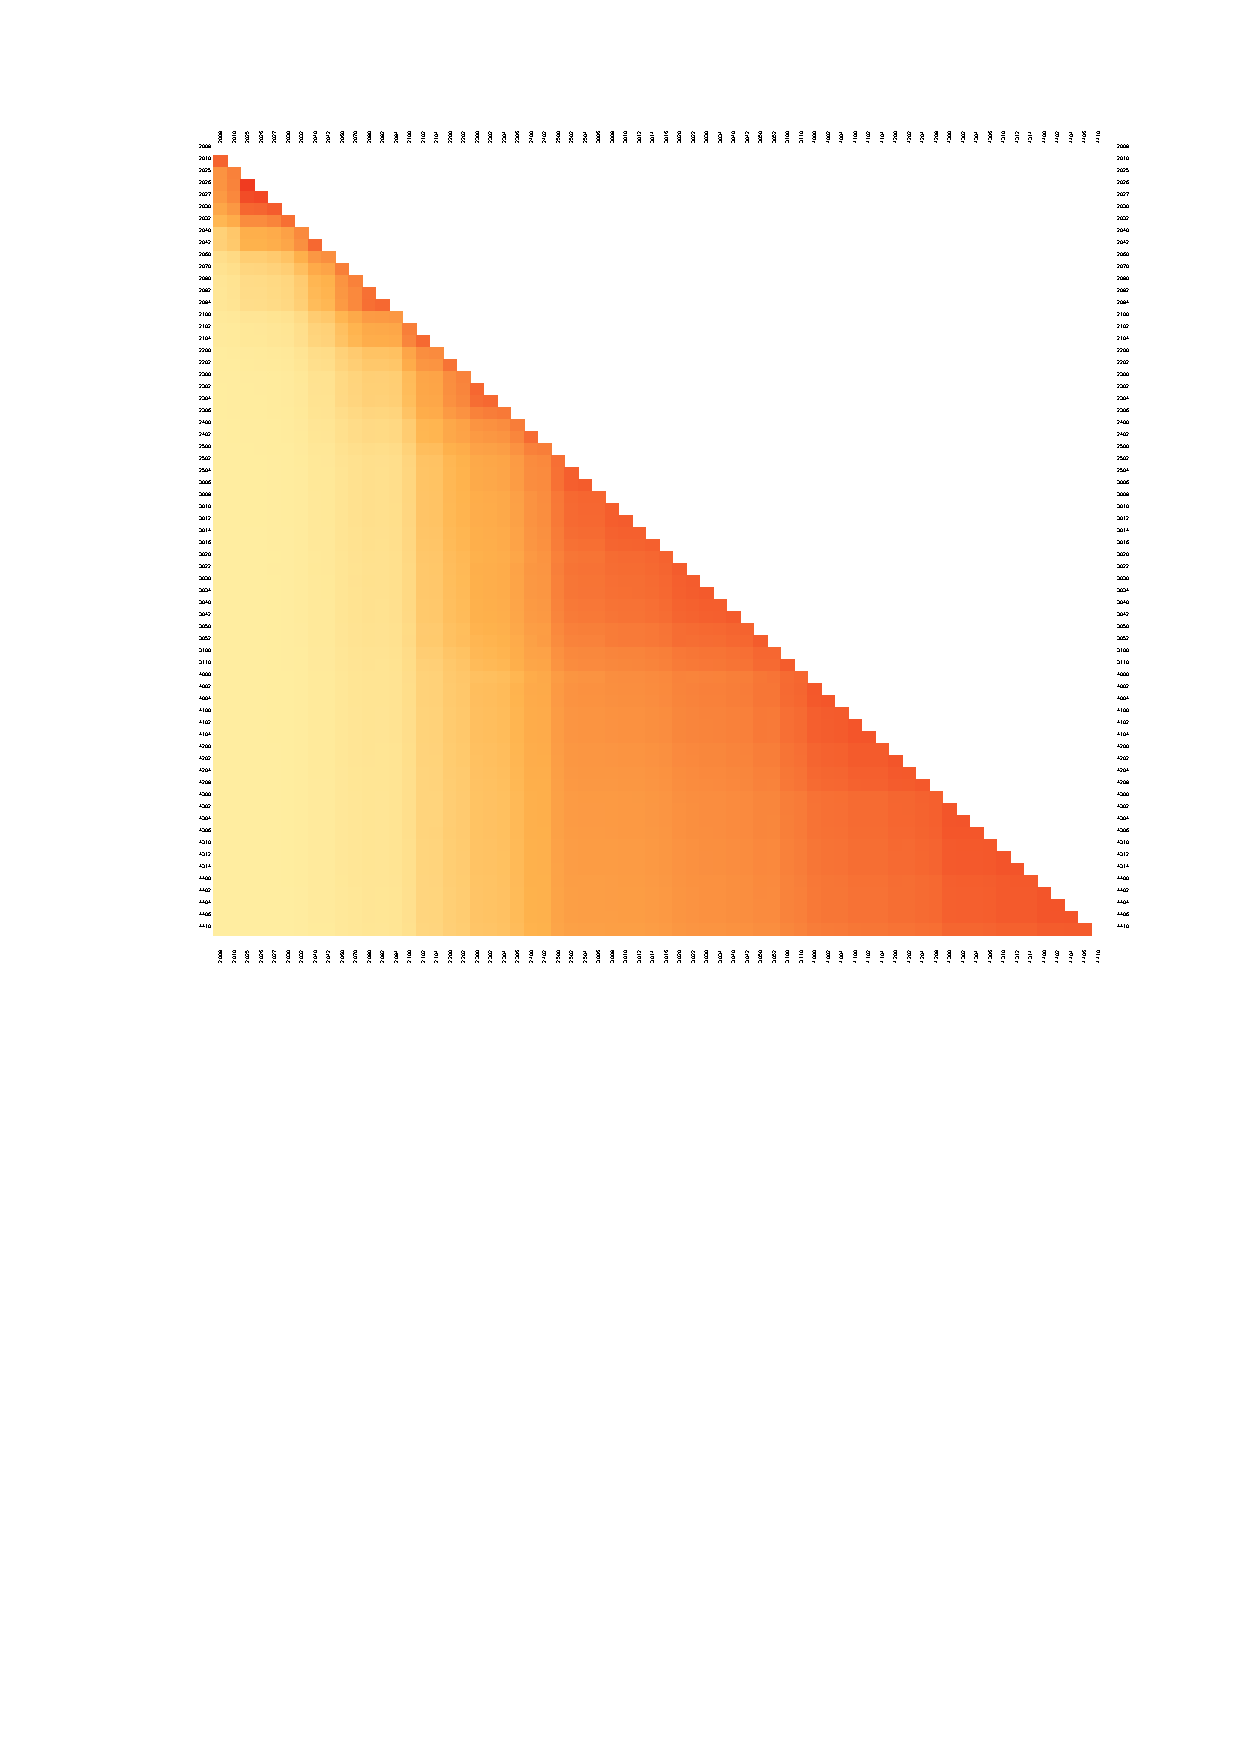
\includegraphics[width=\textwidth]{first66min-max.pdf}
\caption{Heat map of the code clone coverage ratio between different Azureus/Vuze versions.}
\label{fig:min-max}
\end{figure*}

\begin{thebibliography}{9}
\bibitem{paper}
S. Livieri, Y. Higo, M. Matsushita, K. Inoue. \emph{Analysis of the Linux Kernel Evolution Using Code Clone Coverage.} Proceedings of the Fourth International Workshop on Mining Software Repositories (MSR 2007),  pp. 22-1 22-4, Washington, DC, USA, 2007.
\bibitem{CCFinder}
T. Kamiya, S. Kusumoto, K. Inoue. \emph{CCFinder: a multilinguistic token-based code clone detection system for large scale source code.} IEEE Transactions on Software Engineering, Volume 28, Issue 7, pages 654-670, July 2002.
\end{thebibliography}


\onecolumn
\pagestyle{empty} %//TODO empty pagestyle or similar to rest of report?
\begin{appendices}
\section{Bash script}\label{script}
\scriptsize
\begin{verbatim}
#!/bin/bash

#list all folders countaining a version of Azureus/Vuze
folders=$(ls /home/ubuntu/ccfinder-src/source/source)

#loop doing all pairwise comparisons and calculating the metric
for folder in $folders; do
    #determine sloc, as per the paper, with using wc -l.
    sloc[$folder]=$(( find /home/ubuntu/ccfinder-src/source/source/$folder 
        -name '*.java' -print0 | xargs -0 cat) | wc -l)

    #do comparissons
    for folder2 in $folders; do    
        #make sure to triangulate, not rectangulate
        if [ $folder -gt $folder2 ]; then     
            ../ccfx d java -b 50 -dn /home/ubuntu/ccfinder-src/source/source/$folder 
                -is -dn /home/ubuntu/ccfinder-src/source/source/$folder2 -w f-w-g+ 
                    -o $folder-$folder2.ccfxd 

            #filter clone file for RNR < 0.5
            ../ccfx m $folder-$folder2.ccfxd -c -o clone-$folder-$folder2.tsv            
            ../picosel -o toremain-$folder-$folder2.txt from clone-$folder-$folder2.tsv 
                select CID where RNR .ge. 0.5
            ../ccfx s $folder-$folder2.ccfxd -o $folder-$folder2-filtered.ccfxd -ci 
                toremain-$folder-$folder2.txt

            #calculate number of lines per clone
            ../ccfx m $folder-$folder2-filtered.ccfxd -w 
                -o line-$folder-$folder2.tsv 
            cat line-$folder-$folder2.tsv
                |awk 'NR>1{print $4}' > cloc-$folder-$folder2.txt
            Cij=$(paste -sd+ cloc-$folder-$folder2.txt | bc)

            #calculate and perform output
            sumSloc=$((${sloc[$folder]} + ${sloc[$folder2]}))
            coverage=$(echo "scale=10; $Cij/$sumSloc" | bc -l)
            echo $folder$folder2,$coverage >> output.txt

            #remove all temporary created files now
            rm -f $folder-$folder2.ccfxd
            rm -f clone-$folder-$folder2.tsv
            rm -f toremain-$folder-$folder2.txt 
            rm -f $folder-$folder2-filtered.ccfxd
            rm -f line-$folder-$folder2.tsv
            rm -f cloc-$folder-$folder2.txt
            rm -f clone-$folder-$folder2-filtered.tsv
        fi
    done
done



\end{verbatim}
\end{appendices}



\end{document}
